\section{Results}
\label{sec:results}

The evaluation proceeds in two layers: Rust backend attribution (Section~\ref{sec:rust-results}) and vLLM integration (Section~\ref{sec:vllm-results}), with Tensora's Python bindings serving as the bridge between them. Tables present core evidence; figures visualize regime crossovers.

\begin{table}[htbp]
\caption{Regime map: strongest observed explicit backend by layout, environment, and scale. Color encodes the winning backend. The key visual fact is non-dominance: every backend color appears, and the pattern changes with layout and environment.}
\label{tab:regime-map}
\centering
\small
\begin{tabular}{lllll}
\toprule
Layer / layout & 0.6B & 4B & 8B & 32B \\
\midrule
H100 SafeTensors & \syncwin & \syncwin & \uringwin & \uringwin \\
H100 ServerlessLLM & \uringwin & \asyncwin & \uringwin & \asyncwin \\
H200 SafeTensors & \syncwin & \syncwin & \asyncwin & \asyncwin \\
H200 ServerlessLLM & \asyncwin & \asyncwin & \asyncwin & \asyncwin \\
A100 SafeTensors & \syncwin & \asyncwin & \asyncwin & \syncwin \\
A100 ServerlessLLM & \syncwin & \asyncwin & \asyncwin & \asyncwin \\
vLLM SafeTensors & \syncwin & \syncwin & \uringwin & \uringwin \\
\bottomrule
\end{tabular}
\end{table}

Table~\ref{tab:regime-map} is the visual thesis of the paper. SafeTensors begins in the sync regime and shifts with scale. On H100 ServerlessLLM, sync is never the fastest backend. Restricted environments replace \texttt{io\_uring} with async. vLLM preserves the small-versus-large structure. A single fixed backend cannot reproduce this map.

\begin{table}[htbp]
\caption{Effect-size summary for representative regime claims. Ratios are computed as slower time divided by faster time; larger values indicate stronger evidence for a regime distinction.}
\label{tab:effect-summary}
\centering
\small
\begin{tabular}{p{0.42\textwidth}p{0.24\textwidth}p{0.22\textwidth}}
\toprule
Claim & Evidence row & Effect size \\
\midrule
Small SafeTensors favors low-overhead sync over \texttt{io\_uring} & H100 Qwen3-0.6B & sync is 2.09$\times$ faster than \texttt{io\_uring} \\
Large SafeTensors needs deeper submission & H100 Qwen3-32B & \texttt{io\_uring} is 1.28$\times$ faster than sync \\
Partitioning removes sync as winner & H100 ServerlessLLM Qwen3-32B & async is 1.36$\times$ faster than sync \\
\texttt{io\_uring} availability changes large-scale winner & H200 SafeTensors Qwen3-32B & async is 3.41$\times$ faster than sync when \texttt{io\_uring} is blocked \\
Serving impact survives integration & vLLM Qwen3-32B cold load\_only & \texttt{io\_uring} SafeTensors is 48.1\% faster than native \\
\bottomrule
\end{tabular}
\end{table}

\subsection{Headline findings}

Four patterns emerge from the Rust and integration matrices. First, SafeTensors exhibits a scale crossover from sync to \texttt{io\_uring}, while on H100 ServerlessLLM, sync is never the fastest backend. Second, integration overhead reorders but does not erase backend effects: vLLM costs dominate absolute time, yet loader choice still changes cold initialization by tens of seconds at larger scales. Third, ordering regimes transfer better than backend identities: cross-environment validation confirms that small SafeTensors loads favor sync in three of four environments (with async as the gVisor exception on Modal), while the large-scale winner varies with storage topology and kernel capability. Fourth, no single explicit backend wins across the full parameter space.

\subsection{Rust Backend Results}
\label{sec:rust-results}

The Rust harness is the authoritative backend-attribution layer because it measures checkpoint loading directly, without Python tensor conversion or serving-engine initialization costs. Unless stated otherwise, each matrix cell is one representative cold-cache run. Half the matrix (18 of 36 cells) is backed by five-repetition anchor sets with median and range (Appendix~\ref{app:anchor-stats}). Where anchor ranges overlap between backends, we note that the ranking is not statistically separable rather than forcing a strict order. The main regime claims are supported by non-overlapping ranges and large effect sizes.

\subsubsection{SafeTensors Results}

Table~\ref{tab:rust-safetensors} summarises the explicit backend comparison for SafeTensors.

\begin{table}[htbp]
\caption{Rust cold-cache SafeTensors results (ms). The crossover from sync-favored small models to io\_uring-favored large multi-shard models is the clearest regime signal.}
\label{tab:rust-safetensors}
\centering
\begin{tabular}{lrrr}
\toprule
Model & Sync & Async & io\_uring \\
\midrule
Qwen3-0.6B & 555.28 & 1416.19 & 1159.24 \\
SmolLM3-3B & 1331.79 & 5802.05 & 3812.35 \\
Qwen3-4B & 1820.85 & 5039.21 & 2967.42 \\
Qwen3-8B & 3880.40 & 7074.40 & 3172.37 \\
Qwen3-14B & 7030.25 & 13489.00 & 5977.07 \\
Qwen3-32B & 15454.45 & 28763.46 & 12089.05 \\
\bottomrule
\end{tabular}
\end{table}

Two regimes are visible. The small end of the ladder favors low-overhead sync (555~ms over io\_uring's 1159~ms at Qwen3-0.6B). The ranking flips at Qwen3-8B: io\_uring at 3172~ms versus sync at 3880~ms, a 1.22$\times$ advantage. At the largest scale (Qwen3-32B), io\_uring is 1.28$\times$ faster than sync (12089~ms vs 15454~ms). The crossover is not a single threshold; it is a progression visible across the entire ladder.

Anchor data confirms the key claims. At Qwen3-8B, io\_uring's five-repetition range [3160 to 3274~ms] does not overlap sync's [3648 to 3731~ms], confirming a clean regime separation (non-overlapping five-run ranges). At Qwen3-32B, io\_uring [11737 to 14389~ms] is separated from sync [15327 to 16144~ms]. At Qwen3-0.6B the opposite separation is visible: sync [322 to 403~ms] is well below io\_uring [1156 to 1264~ms], confirming the small-scale sync regime across all three backends.

Async is consistently the weakest backend for SafeTensors. Whole-file and multi-shard loads benefit from straightforward bulk parallelism rather than scheduler-mediated async orchestration, which adds overhead without corresponding I/O benefits on this workload shape.

\begin{figure}[htbp]
    \centering
    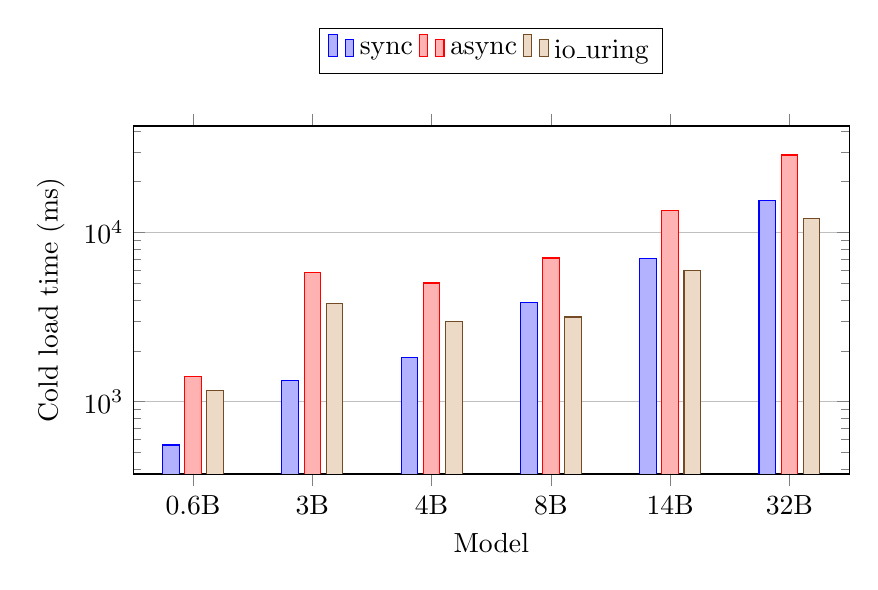
\begin{tikzpicture}
    \begin{axis}[
    width=0.88\textwidth,
    height=6cm,
    ybar,
    bar width=6pt,
    ymode=log,
    ylabel={Cold load time (ms)},
    xlabel={Model},
    symbolic x coords={0.6B,3B,4B,8B,14B,32B},
    xtick=data,
    legend style={at={(0.5,1.15)},anchor=south,legend columns=4},
    ymajorgrids=true,
    every axis plot/.style={fill=gray!40,draw=black},
    ]
    \addplot coordinates {(0.6B,555.28) (3B,1331.79) (4B,1820.85) (8B,3880.40) (14B,7030.25) (32B,15454.45)};
    \addplot coordinates {(0.6B,1416.19) (3B,5802.05) (4B,5039.21) (8B,7074.40) (14B,13489.00) (32B,28763.46)};
    \addplot coordinates {(0.6B,1159.24) (3B,3812.35) (4B,2967.42) (8B,3172.37) (14B,5977.07) (32B,12089.05)};
    \legend{sync,async,io\_uring}
    \end{axis}
    \end{tikzpicture}
    \caption{SafeTensors backend crossover (log scale). Sync dominates small models; io\_uring dominates large multi-shard models.}
    \label{fig:safetensors-crossover}
\end{figure}

Figure~\ref{fig:safetensors-crossover} visualizes the progression from sync-favored to io\_uring-favored loading.

\subsubsection{ServerlessLLM-style Partitioned-layout Results}

The ServerlessLLM layout produces a different ordering, shown in Table~\ref{tab:rust-serverlessllm}.

\begin{table}[htbp]
\caption{Rust cold-cache ServerlessLLM results (ms). Synchronous loading never wins; the ranking shifts from async at smaller partition scales toward io\_uring at larger sizes.}
\label{tab:rust-serverlessllm}
\centering
\begin{tabular}{lrrr}
\toprule
Model & Sync & Async & io\_uring \\
\midrule
Qwen3-0.6B & 1645.06 & 1471.34 & 1387.57 \\
SmolLM3-3B & 3941.88 & 2391.24 & 3091.49 \\
Qwen3-4B & 5137.72 & 3504.25 & 3727.14 \\
Qwen3-8B & 11048.40 & 9463.37 & 9043.51 \\
Qwen3-14B & 18661.25 & 16139.08 & 13257.23 \\
Qwen3-32B & 39822.09 & 29180.89 & 29779.86 \\
\bottomrule
\end{tabular}
\end{table}

Sync is the slowest explicit backend on every ServerlessLLM row, between 1.1$\times$ (Qwen3-0.6B) and 1.4$\times$ (Qwen3-32B) behind the strongest alternative. The best explicit backend varies with scale: async dominates at smaller partition counts (SmolLM3-3B, Qwen3-4B), while io\_uring becomes competitive at larger scales (Qwen3-14B, Qwen3-32B).

Anchor data reveals important nuance. At ServerlessLLM Qwen3-0.6B, async [1331 to 1409~ms] and io\_uring [1395 to 1483~ms] have overlapping ranges; the ranking between non-sync backends is not always statistically separable. At Qwen3-8B, io\_uring [7119 to 8885~ms] and async [7628 to 9837~ms] overlap; only sync [10175 to 10676~ms] is clearly separated as slowest. At Qwen3-32B, io\_uring [26664 to 29152~ms] and async [28639 to 29222~ms] overlap; again, only sync [37785 to 40691~ms] is cleanly separated. The consistent structural fact, that sync loses on every ServerlessLLM row, is robustly confirmed; the ordering among non-sync backends at individual scales is closer and less stable.

\begin{figure}[htbp]
    \centering
    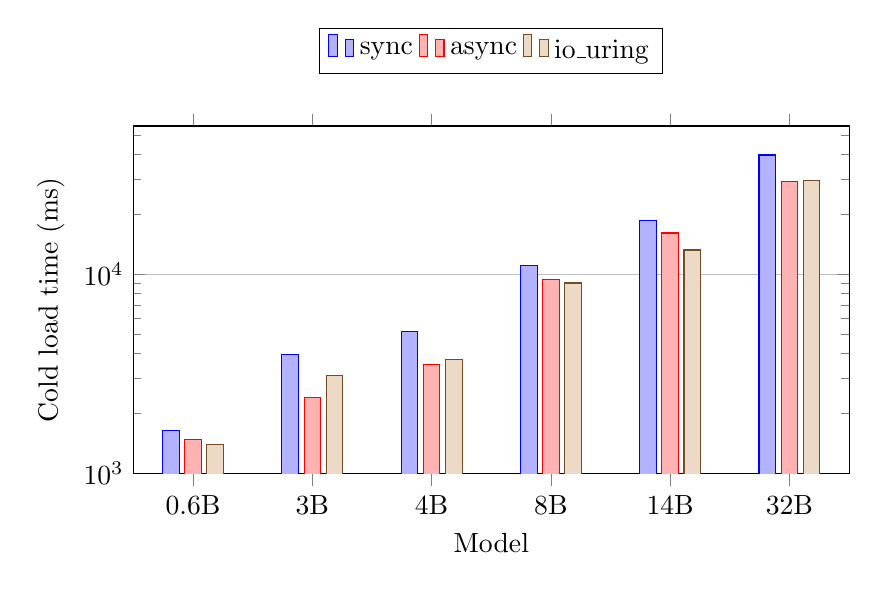
\begin{tikzpicture}
    \begin{axis}[
    width=0.88\textwidth,
    height=6cm,
    ybar,
    bar width=6pt,
    ymode=log,
    ylabel={Cold load time (ms)},
    xlabel={Model},
    symbolic x coords={0.6B,3B,4B,8B,14B,32B},
    xtick=data,
    legend style={at={(0.5,1.15)},anchor=south,legend columns=4},
    ymajorgrids=true,
    every axis plot/.style={fill=gray!40,draw=black},
    ]
    \addplot coordinates {(0.6B,1645.06) (3B,3941.88) (4B,5137.72) (8B,11048.40) (14B,18661.25) (32B,39822.09)};
    \addplot coordinates {(0.6B,1471.34) (3B,2391.24) (4B,3504.25) (8B,9463.37) (14B,16139.08) (32B,29180.89)};
    \addplot coordinates {(0.6B,1387.57) (3B,3091.49) (4B,3727.14) (8B,9043.51) (14B,13257.23) (32B,29779.86)};
    \legend{sync,async,io\_uring}
    \end{axis}
    \end{tikzpicture}
    \caption{ServerlessLLM backend ordering (log scale). Sync is never the winner; the ranking shifts toward async and io\_uring.}
    \label{fig:serverlessllm-crossover}
\end{figure}

Figure~\ref{fig:serverlessllm-crossover} shows that the ServerlessLLM workload shape (many small range reads across partition files) rewards different backends than the SafeTensors contiguous regime.

\subsection{Backend Non-Dominance Summary}

Three findings summarize the backend comparison. First, SafeTensors has a clean crossover: sync dominates at small scale and \texttt{io\_uring} at large scale on H100. Second, H100 ServerlessLLM removes sync as a winner; async and \texttt{io\_uring} trade places by partition scale. Third, no single backend wins across both layouts, a direct designer-facing implication.

\subsection{Cross-Environment Validation}
\label{sec:cross-env}

The H100 results above were collected with all three backends available, including \texttt{io\_uring}. Two additional environments (an H200 container and an A100 container, both with network-attached storage) block \texttt{io\_uring} at the kernel level (\texttt{EPERM}). This constraint tests whether ordering regimes transfer across hardware when the strongest H100 backend is unavailable.

The regime structure (backend ordering as a function of format and scale) persists: small SafeTensors loads favor sync on H100, H200, and A100, while on Modal H100 under gVisor async wins at small scale due to gVisor's per-syscall overhead penalizing synchronous I/O more than batched async submission. The mid-to-large-scale winner changes with storage topology and kernel capability: \texttt{io\_uring} on local NVMe (H100), async on network storage (H200), and sync recovering at the largest A100 scale. Complete cross-environment matrices appear in Appendix~\ref{app:cross-env}.

Held-out validation on Mistral-7B-Instruct (Appendix~\ref{app:held-out}), a different architecture family with different shard geometry, confirms that the structural regime claims generalize beyond the primary model ladder: sync is never fastest for ServerlessLLM on either model. The SafeTensors pattern is geometry-dependent: async dominates the 5-shard Qwen3-8B by 2.92$\times$, while sync remains fastest on Mistral-7B's 3-shard layout, consistent with the finding that low-shard-count SafeTensors loads favor low-overhead backends.

\subsection{vLLM Results}
\label{sec:vllm-results}

The final vLLM matrix completed successfully across all six models, all benchmark loaders, warm and cold cache conditions, and all three benchmark kinds.

\textbf{Stock vLLM versus Tensora.} The \texttt{native} loader follows vLLM's default weight-loading path; \texttt{ts\_*} loaders use Tensora-backed integrations. Table~\ref{tab:vllm-full-cold} shows the complete cold \texttt{load\_only} matrix across all six models. On cold \texttt{load\_only}, Tensora's SafeTensors loader family reduces initialization time relative to \texttt{native} across all scales.

\begin{table}[htbp]
\caption{Cold vLLM load\_only across all models and loader families (ms). Tensora's SafeTensors explicit backends consistently outperform native. ServerlessLLM paths improve over native on large models.}
\label{tab:vllm-full-cold}
\centering
\resizebox{\linewidth}{!}{%
\small
\begin{tabular}{lrrrrrr}
\toprule
Model & \texttt{native} & \texttt{ts\_st\_sync} & \texttt{ts\_st\_iour} & \texttt{ts\_sllm\_sync} & \texttt{ts\_sllm\_iour} \\
\midrule
Qwen3-0.6B & 23659 & 20417 & 20867 & 21191 & 21262 \\
SmolLM3-3B & 36874 & 27767 & 29992 & 30870 & 30287 \\
Qwen3-4B & 40486 & 28478 & 29727 & 32327 & 31792 \\
Qwen3-8B & 56639 & 36524 & 35889 & 44371 & 42343 \\
Qwen3-14B & 89220 & 49435 & 47751 & 63150 & 61848 \\
Qwen3-32B & 169971 & 92421 & 88164 & 124049 & 111717 \\
\bottomrule
\end{tabular}%
}
\end{table}

The improvement grows with model size: at Qwen3-32B, Tensora's SafeTensors \texttt{io\_uring} reduces initialization by 48.1\% relative to native (88164~ms vs 169971~ms). This is consistent with the Rust SafeTensors finding that \texttt{io\_uring}'s advantage grows with scale. The ServerlessLLM paths also improve over native at large scales (34\% reduction at 32B) but trail SafeTensors paths by 21 to 34\%, consistent with the Rust finding that partitioned range layouts have higher overhead.

For cold load\_only across all models, the best loader varies with model size. Table~\ref{tab:vllm-load-only} shows the strongest loader in the final cold-load-only configuration.

\begin{table}[htbp]
\caption{Best cold load\_only vLLM loader by model. The pattern follows the Rust SafeTensors regime: sync at small scales, io\_uring at large scales.}
\label{tab:vllm-load-only}
\centering
\begin{tabular}{lrl}
\toprule
Model & Best init time (ms) & Best loader \\
\midrule
Qwen3-0.6B & 20417 & ts\_safetensors\_sync \\
SmolLM3-3B & 27767 & ts\_safetensors\_sync \\
Qwen3-4B & 28478 & ts\_safetensors\_sync \\
Qwen3-8B & 35889 & ts\_safetensors\_io\_uring \\
Qwen3-14B & 47751 & ts\_safetensors\_io\_uring \\
Qwen3-32B & 88164 & ts\_safetensors\_io\_uring \\
\bottomrule
\end{tabular}
\end{table}

The vLLM best-loader pattern mirrors the Rust SafeTensors crossover: smaller models favor sync, larger models favor io\_uring. The match is not exact (vLLM initialization includes fixed costs that dilute the pure-I/O ranking), but the regime structure survives.

For TTFT, the ranking follows load\_only but the proportional advantage shrinks. At Qwen3-32B, ts\_safetensors\_io\_uring TTFT (89259~ms median) is 41.3\% lower than native (152184~ms median); the load\_only reduction at the same model was 48.1\%. The smaller TTFT improvement reflects the first-generation compute step diluting the I/O savings. The SafeTensors loader family consistently outperforms ServerlessLLM for both metrics. Load\_only and TTFT show backend effects mainly in initialization; decode is comparatively insensitive once weights are resident.

\subsection{Layer summary}

Four principles emerge. (1) Backend ranking depends on workload shape: SafeTensors favors sync at small scale and \texttt{io\_uring} at large H100 scale, while on H100 ServerlessLLM, sync is never the fastest backend. (2) Integration layers reorder but do not eliminate backend differences: vLLM adds engine initialization cost that compresses proportional spreads, yet backend choice still changes user-visible startup. (3) Cross-environment validation confirms that small SafeTensors loads favor sync on H100, H200, and A100 (with Modal H100 as the gVisor exception where async wins at small scale); the mid-to-large-scale winner varies with kernel interface availability and storage topology. (4) No single explicit backend dominates the full parameter space; loader design should therefore expose backend choice and regime awareness.
